\thispagestyle{main}
\chapter{Latex部分代码示例}
\thispagestyle{main}


\section{一些有用的工具}

LaTeX基本命令使用教程:https://blog.csdn.net/gentleman\_qin/article/details/79963396。

在线表格可视化网站:https://tablesgenerator.com/。

在线公式生成网站:https://www.latexlive.com/home。


\section{图片}

\subsection{单张图片示例}

\textbf{注意,图片的标题在下面。}
\begin{figure}[!ht]
    \centering
    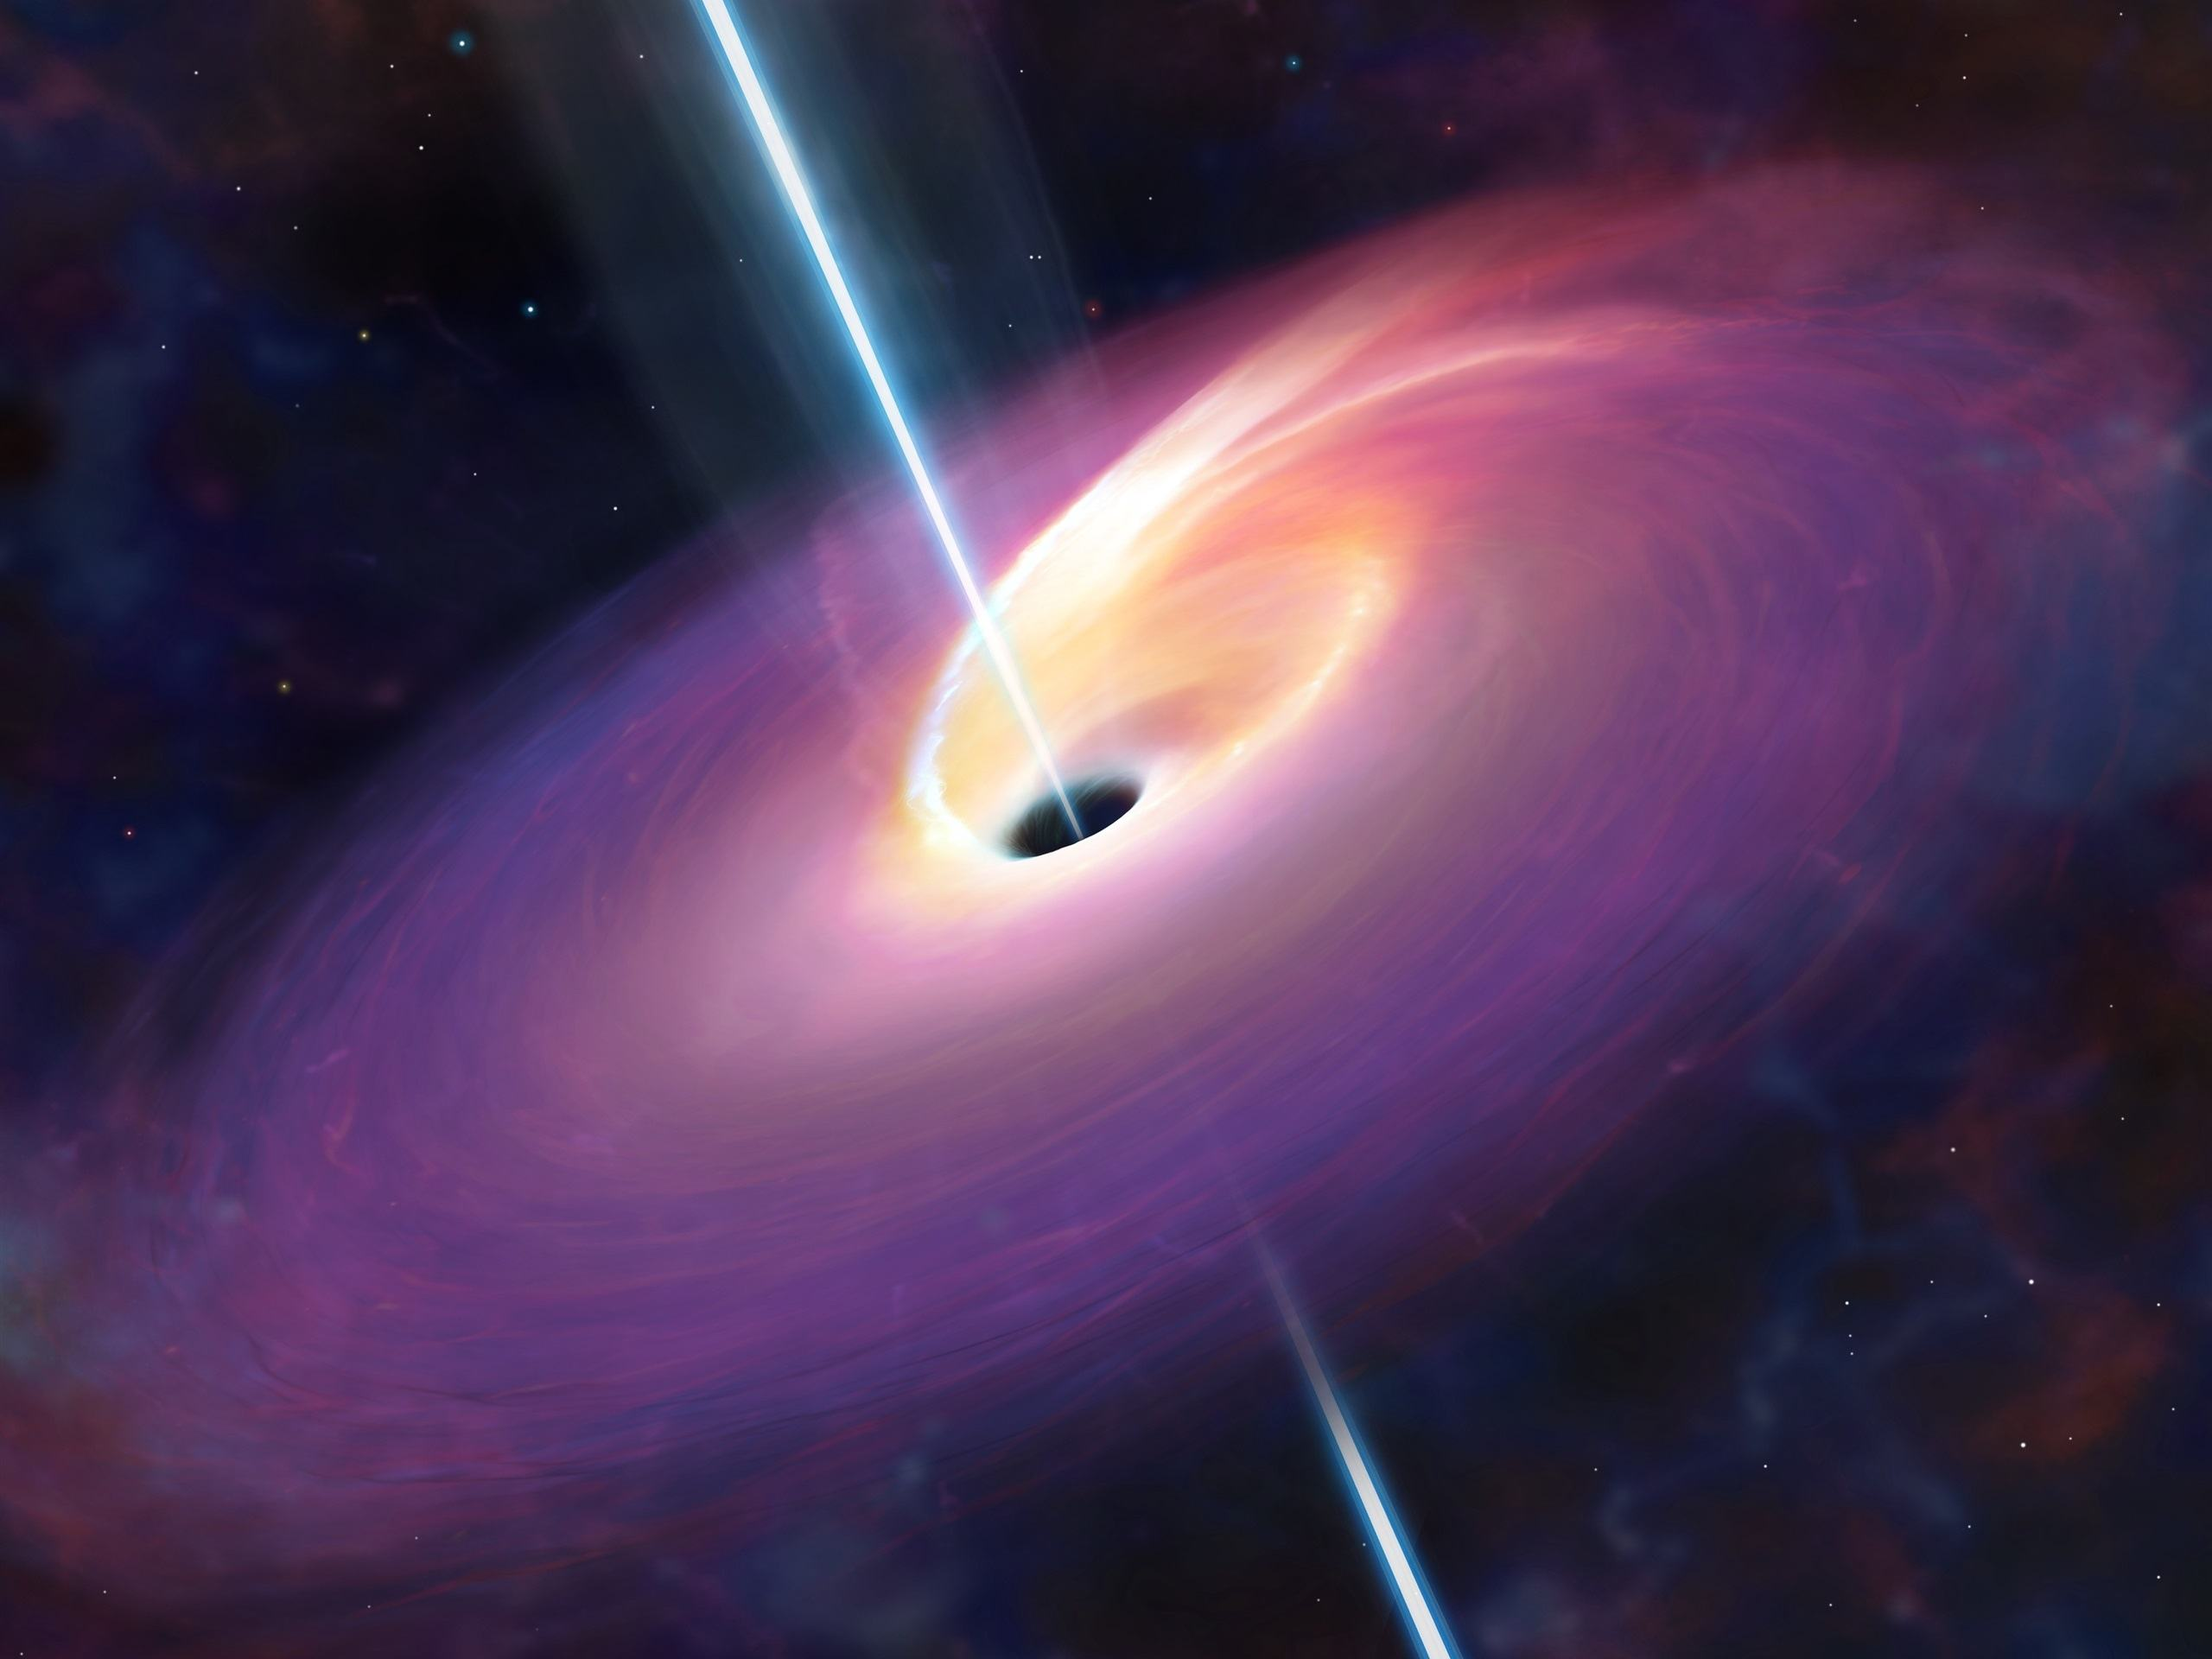
\includegraphics[width=2.5in]{images/blackhole.jpeg}
    \caption{黑洞}
    \label{fig:blackhole1}
\end{figure}
图~\ref{fig:blackhole1}是单个黑洞图片。

\subsection{多张图片示例}

\begin{figure*}[!ht]
    \centering
    \subfloat[图片1。]{
        \includegraphics[width = 0.45\textwidth]{example-image}
    }
    \hfill
    \subfloat[图片2]{
        \includegraphics[width = 0.45\textwidth]{example-image}
    }
    \\
    \subfloat[图片3。]{
        \includegraphics[width = 0.45\textwidth]{example-image}
    }
    \hfill
    \subfloat[图片4。]{
        \includegraphics[width = 0.45\textwidth]{example-image}
    }
    \caption{多个黑洞}
    \label{fig:blackhole2}
\end{figure*}
图~\ref{fig:blackhole2}是多个黑洞图片并列。


\section{表格}

\textbf{注意,表格的标题在上面。}
\begin{table}[!ht]
\centering
\caption{一个表的实例}
\begin{tabular}{cccccc}
    \toprule
    序号 & 姓名 & 性别 & 年龄 & 身高/cm & 体重/kg \\
    \midrule
    1 & 张三 & M & 16 & 163 & 50 \\
    2 & 王红 & F & 15 & 159 & 47 \\
    3 & 李二 & M & 17 & 165 & 52 \\
    \bottomrule
\end{tabular}
\label{tab:tabobj}
\end{table}
表~\ref{tab:tabobj}是一个实例。


\section{简单的数学公式和定理}

\begin{sthm}[定理~\thethm~(存在性定理)]
    $\Gamma\Theta\Lambda\Xi\Pi\alpha\beta\gamma\delta$
\end{sthm}

\begin{thm}
\label{thm:alpha}
    xxxxx
\end{thm}

\begin{equation}
\label{eq:alpha}
    \alpha=\sqrt[n]{\Re}.
\end{equation}
定理\ref{thm:alpha},公式\ref{eq:alpha}。


\section{伪代码实例}

\subsection{使用algorithmic包}

\begin{algorithm}[!ht]
\caption{algorithmic示例}
\begin{algorithmic}[1] %[1] 能够显示行号
    \REQUIRE $n \geq 1$                  %输入条件
    \ENSURE $Sum = 1 + \cdots + n$       %输出
    \STATE $Sum \leftarrow 0$            %\STATE 命名演示
    \IF {$n < 1$}                        %条件语句
        \PRINT {Input Error}                 %打印语句
    \ELSE
        \FOR {$i = 0$ to n}          %FOR循环结构
            \STATE $Sum = Sum + i$\\
            \STATE $i = i + 1$
        \ENDFOR
    \ENDIF
    \RETURN $Sum$
\end{algorithmic}
\label{alg}
\end{algorithm}

算法\ref{alg}表示前n个数字的累加。


\section{枚举列表}

\subsection{普通列表}

\begin{itemize}
    \item 列表项目1;
    \item 列表项目2;
    \item 列表项目3。
\end{itemize}

\subsection{有序列表}

\begin{enumerate}
    \item 有序列表项目1;
    \item 有序列表项目2;
    \item 有序列表项目3。
\end{enumerate}


\section{脚注}

脚注示例\footnote{这是脚注示例。}。


\section{文献引用}

默认的参考文献引用方法是$\backslash$cite\{\}~\cite{broder1997resemblance,broder1997syntactic},也可以使用非上标的引用形式$\backslash$norcite\{\}~\norcite{broder1997resemblance}。


\section{关于参考文献的一些格式问题}

\subsection{关于中文文献的引用}

对于中文文献,建议增加参数“language={zh}”。对于超过3个作者以上的中文参考文献,第四位及以后的作者需要被省略,并增加“等”字。这个参数能够规避中文参考文献中出现“et al.”的错误。

例如接下来的这个文献:
@article\{郑一力2017,
  title=\{基于多特征降维的植物叶片识别方法\},
  author=\{郑一力 and 钟刚亮 and 王强 and 赵玥 and 赵燕东\},
  journal=\{农业机械学报\},
  volume=\{48\},
  number=\{3\},
  pages=\{30--37\},
  year=\{2017\},
  \textbf{language=\{zh\}}
\}

\subsection{关于英文姓名的大小写问题}

部分用户曾反馈,\textbf{为什么参考文献中的作者的名全部是大写?}
不得不承认,仅首字母大写的书写方式更加好看。但根据中国国家标准《GB/T 7714-2015: 信息与文献 参考文献著录规则》,名的全部大写才是符合规范的。因此,本项目将继续以该国标作为标准进行完善。

考虑到部分同学可能有特殊需要,如果希望格式改成首字母大写其余小写的形式,可以在gbt7714-2015.bst文件中第637行的“"u" change.case\$ 'lastname :=”改成“"t" change.case\$ 'lastname :=”即可。

在本条目更新之前,一些同学已经发现了这个小诀窍,为他们的聪明才智鼓掌。


\section{关于图、表标题的一些其他应用}

如果在图片、表格的标题中需要用到较长的内容解释结果,或者内容中包含引用,建议使用``$\backslash$caption[<短标题>]\{<长标题>\}''命令。可选的参数短标题用于图表目录,而长标题中可以进行长达多段的叙述。而标签$\backslash$label需要放在caption后面,或者短标题或长标题中。实际效果如下表所示:

\begin{table}[!t]
\centering
\caption[这是表目录中的标题]{这是正文中表格的标题,也可以正常使用引用论文\cite{broder1997resemblance}。}
\begin{tabular}{ccc}
    \toprule
    序号 & 姓名 & 薪水 \\
    \midrule
    1 & Mark    & $\$5,000$   \\
    2 & Carly   & $\$8,000$    \\
    3 & Carter  & $\$6,500$    \\
    \bottomrule
\end{tabular}
\\
\begin{flushleft}
\wuhao 注:这是注释,可以对图或者表进行更多的解释。
\end{flushleft}
\label{tab:example}
\end{table}
在表~\ref{tab:example}中,引用如果放在了短标题中,会在正文前先对引用进行编号,导致引用排序出现问题,望知晓。

此外,部分作者可能会遇到需要对图或表进行更详细说明的情况。在这个示例中,增加了文本框以实现对表格的更多解释,供同学们参考。
